%!BIB TS-program = biber
\documentclass[11pt]{article}%
\usepackage{amsmath}
\usepackage{amsfonts}
\usepackage{amssymb,tcolorbox}
\usepackage{graphicx}
\usepackage{amssymb}%
\usepackage{siunitx}
\usepackage{listings}
\usepackage[style=ieee]{biblatex}
\setcounter{MaxMatrixCols}{30}
\providecommand{\U}[1]{\protect\rule{.1in}{.1in}}
\providecommand{\U}[1]{\protect\rule{.1in}{.1in}}
\providecommand{\U}[1]{\protect\rule{.1in}{.1in}}
\newtheorem{theorem}{Theorem}
\newtheorem{acknowledgement}[theorem]{Acknowledgement}
\newtheorem{algorithm}[theorem]{Algorithm}
\newtheorem{axiom}[theorem]{Axiom}
\newtheorem{case}[theorem]{Case}
\newtheorem{claim}[theorem]{Claim}
\newtheorem{conclusion}[theorem]{Conclusion}
\newtheorem{condition}[theorem]{Condition}
\newtheorem{conjecture}[theorem]{Conjecture}
\newtheorem{corollary}[theorem]{Corollary}
\newtheorem{criterion}[theorem]{Criterion}
\newtheorem{definition}[theorem]{Definition}
\newtheorem{example}[theorem]{Example}
\newtheorem{exercise}[theorem]{Exercise}
\newtheorem{lemma}[theorem]{Lemma}
\newtheorem{notation}[theorem]{Notation}
\newtheorem{problem}[theorem]{Problem}
\newtheorem{proposition}[theorem]{Proposition}
\newtheorem{remark}[theorem]{Remark}
\newtheorem{solution}[theorem]{Solution}
\newtheorem{summary}[theorem]{Summary}
\newenvironment{proof}[1][Proof]{\noindent\textbf{#1.} }{\ \rule{0.5em}{0.5em}}
\addtolength{\oddsidemargin}{-.875in}
\addtolength{\evensidemargin}{-.875in}
\addtolength{\textwidth}{1.75in}
\addtolength{\topmargin}{-1in}
\addtolength{\textheight}{2in}
\usepackage{tocloft}
\usepackage{color} %red, green, blue, yellow, cyan, magenta, black, white
\definecolor{mygreen}{RGB}{28,172,0} % color values Red, Green, Blue
\definecolor{mylilas}{RGB}{170,55,241}

\addbibresource{ndoreport1.bib}

\title{MANE 6710 - Numerical Design Optimization Lab 1}
\author{Human 6966}
\date{September 24 2024}

\renewcommand{\contentsname}{Table of Contents:}
\setcounter{tocdepth}{2} % Include sections and subsections
\setlength{\cftbeforesecskip}{0.5cm} % Adjust spacing between entries
\begin{document}
\maketitle
\newpage
\tableofcontents
\newpage
\addcontentsline{toc}{section}{Executive Summery}
\section*{Executive Summery}
\label{sec:abstract}
Heat exchangers are an important part of many modern systems from home air conditioning and heating, to car engines, to industrial processing facilities and power plants. Heat exchangers are so ubiquitous because they allow for the transfer of heat from one fluid to another without the fluids mixing. This is important because it allows for the design of modular closed-system heaters and coolers (no mass moves in or out of the system) that can affect other systems when coupled. This enables the design problems for complex systems to be broken down into the simpler design problems of subsystems. This lab focuses on choosing and using optimization algorithms in Matlab (\lstinline{fmincon()}) to optimize the profile of a heat exchanger to transfer hear from hot water to air.  A two-dimensional discretized version of Fourier's law was chosen to analyze the thermodynamic system, and the SQP algorithm for \lstinline{fmincon()} was chosen to optimize the profile of the heat exchanger. The SQP algorithm was successfully able to optimize the heat exchanger within the problem constraints by maximizing the area of the heat exchanger touching the air.
\section{Analysis Introduction}
\label{sec:intro}
\subsection {Methodology}
\label{sec:analysismethod}
To analyze the steady-state heat flux per unit length through the heat exchanger, the two-dimensional heat equation (Equation \ref{eqn:delFourier}) was used to find the temperature gradient through the heat exchanger.
\begin{equation}
\label{eqn:delFourier}
\nabla (k\nabla T)=0, \forall x \in \Omega
\end{equation}
 With the boundary conditions:
\begin{equation*}
T(x,y=0)=T_{bottom}
\end{equation*}
\begin{equation*}
T(x,y(x))=T_{top}
\end{equation*}
\begin{equation*}
T(x,y)=T(x+L,y)
\end{equation*}
To solve this equation numerically, Equation \ref{eqn:delFourier} was approximated using a finite-Volume discretization with a unit length resulting in Equation \ref{eqn:descdelFourier}. Which when applied to a mesh, can be used to solve for the temerature gradient.
 \begin{equation}
\label{eqn:descdelFourier}
\int\int_{V}\nabla (k\nabla T)dV\approx\sum_{i=0}^{N_{x}-1}\sum_{j=0}^{N_{y}} k\frac{T_{i+1,j}-T_{i,j}}{\Delta x}\Delta y=0
\end{equation}
From this temperature gradient, the heat flux/unit length could be calculated for the inlet surface using Fourier's law of conduction at $y=0$ (Equation \ref{eqn:heatflux}).
\begin{equation}
\label{eqn:heatflux}
q=\int_{A} k\nabla T \vec{n}dA\approx\sum_{i=0}^{N_{x}-1} k\frac{T_{i+1,0}-T_{i,0}}{\Delta x}\Delta y
\end{equation}
\subsection{Assumptions}
\label{sec:assumption}
To simplify the physical model and fundamental equations, the following assumptions were made:
\begin{enumerate}
   	 \item Constant water temperature in contact with the heat exchanger ($T_{water}=90\si{\degreeCelsius)}$
    	\item Constant air temperature in contact with heat exchanger boundary ($T_{air}=20\si{\degreeCelsius)}$
	\item The temperature of the surface of the heat exchanger is the same as the fluid it is in contact with:
	\begin{itemize}
		\item $T_{top}=T_{air}$
		\item $T_{bottom}=T_{water}$
	\end{itemize}
	\item The heat exchanger is made of a steel alloy with a thermal conductivity of 20 W/(mK)
	\item Steady state heat transfer
	\item Negligable edge effects
	\item  No temperature gradient along the extruded length of the heat exchanger
	\item No heat produced by the heat exchanger
\end{enumerate}
\subsection{Limitations}
These assumptions limit this analysis method to static systems where any protrusions from the surface of the heat exchanger are sufficiently far apart to prevent the temperature of the fluids between them from changing relative to the rest of the fluid. Additionally, the model doesn’t consider convection, so it only works when you know the temperature of both sides of the heat exchanger. Finally, the assumptions about constant fluid temperature, no temperature gradient along the extrusion direction, and negligible edge effects introduce error into the analysis, as these conditions would not be met under real-world circumstances.
\section{Parameterization of the Geometry}
\label{sec:parameterization}
The function chosen to define the shape of the top of the heat exchanger was
\begin{equation}
\label{eqn:hx}
h(x)=a_{0} +\sum_{k=1}^{n}a_{k}sin(\frac{2\pi kx}{L})
\end{equation}
because the function is smooth, periodic, and has many possible shapes. Equation \ref{eqn:hx} was then discretized into a two-dimensional mesh using Equation \ref{eqn:Hij}. 
\begin{equation}
\label{eqn:Hij}
H(i,j)=h(i\frac{L}{N_{x}})\frac{j}{Ny}
\end{equation}
\section{Optimization Method and Limitations}
\label{sec:optimizationmethod}
The SQP (Sequential Quadratic Programming) Algorithm was chosen for \lstinline{fmincon()} (Matlab's nonlinear optimization problem solver \cite{matlab}) to solve the minimization problem. The SQP algorithm uses a quasi-Newton update method to approximate the Hessian, which is used to solve the quadratic subproblems, which are linearized around the current state. Then the algorithm does a line search to determine the step size in the direction of the solution for each node in the mesh. The algorithm iterates through the updated states until the solutions to the quadratic subproblems converge into a smooth gradient. To perform this analysis, the following assumptions were made:
\begin{enumerate}
	\item Constraints are continuously twice differentiable
	\item The objective function is continuously twice differentiable
	\item There is a 'good' initial guess
	\item There is a 'good' mesh
\end{enumerate}
The methodology and assumptions impose the following limitations on this analysis method:
\begin{enumerate}
	\item Due to the derivative assumptions, smooth objective  and model functions are required
	\item Due to ending conditions, a smooth mesh is required
	\begin{itemize}
		\item No discontinuities can be in the mesh
		\item The mesh must be fine enough to capture the gradient 
	\end{itemize}
	\item Due to the gradient-driven update method, the solution may not recover from a step outside the constraints
	\begin{itemize}
		\item Initial guess should start solver inside constraints (algorithm may or may not work otherwise)
		\item A 'bad' step can put algorithm outside constraints
	\end{itemize}
	\item The algorithm won't know if the minimum it found is a local or global minimum 
	\item If the objective function behavior cannot be adequately captured in a localized linear model, this can create ’bad’ steps due to deviation between actual and linearized models
\end{enumerate}

\section{Optimization Problem}
\label{sec:problem}
The objective of this lab is to apply the priciples learned in lecture to optimize the shape of a simple heat exchanger model within the following criteria and constraints\cite{lab1doc}:
\begin{enumerate}
	\item The design is to be two-dimensional and:
	\begin{itemize}
		\item  Can be smoothly repeated horizontally to get heat exchangers of desired widths
		\item Has a width of L = 5 cm (Figure \ref{fig:hxintro1})
	\end{itemize}
	\item The heat exchanger should heat air using hot water
	\begin{itemize}
		\item The steady-state temperature of the water is 90\si{\degreeCelsius}
		\item The steady-state temperature of the air is 20\si{\degreeCelsius}
	\end{itemize}
	\item The side of the heat exchanger that touches the water is flat and will not be altered.
	\item The air-side shape can take on any shape provided:
	\begin{itemize}
		\item The shape is a function of horizontal distance 
		\item The thickness of the heat exchanger is at least 1 cm at any point along the horizontal (Figure \ref{fig:hxintro1} $h_{min}$)
		\item The thickness of the heat exchanger is no more than 5 cm at any point along the horizontal (Figure \ref{fig:hxintro1} $h_{max}$)
		\item The shape is accurately captured by the heat-flux analysis method.
	\end{itemize}
\end{enumerate}
\begin{figure}[h!]
    \centering
    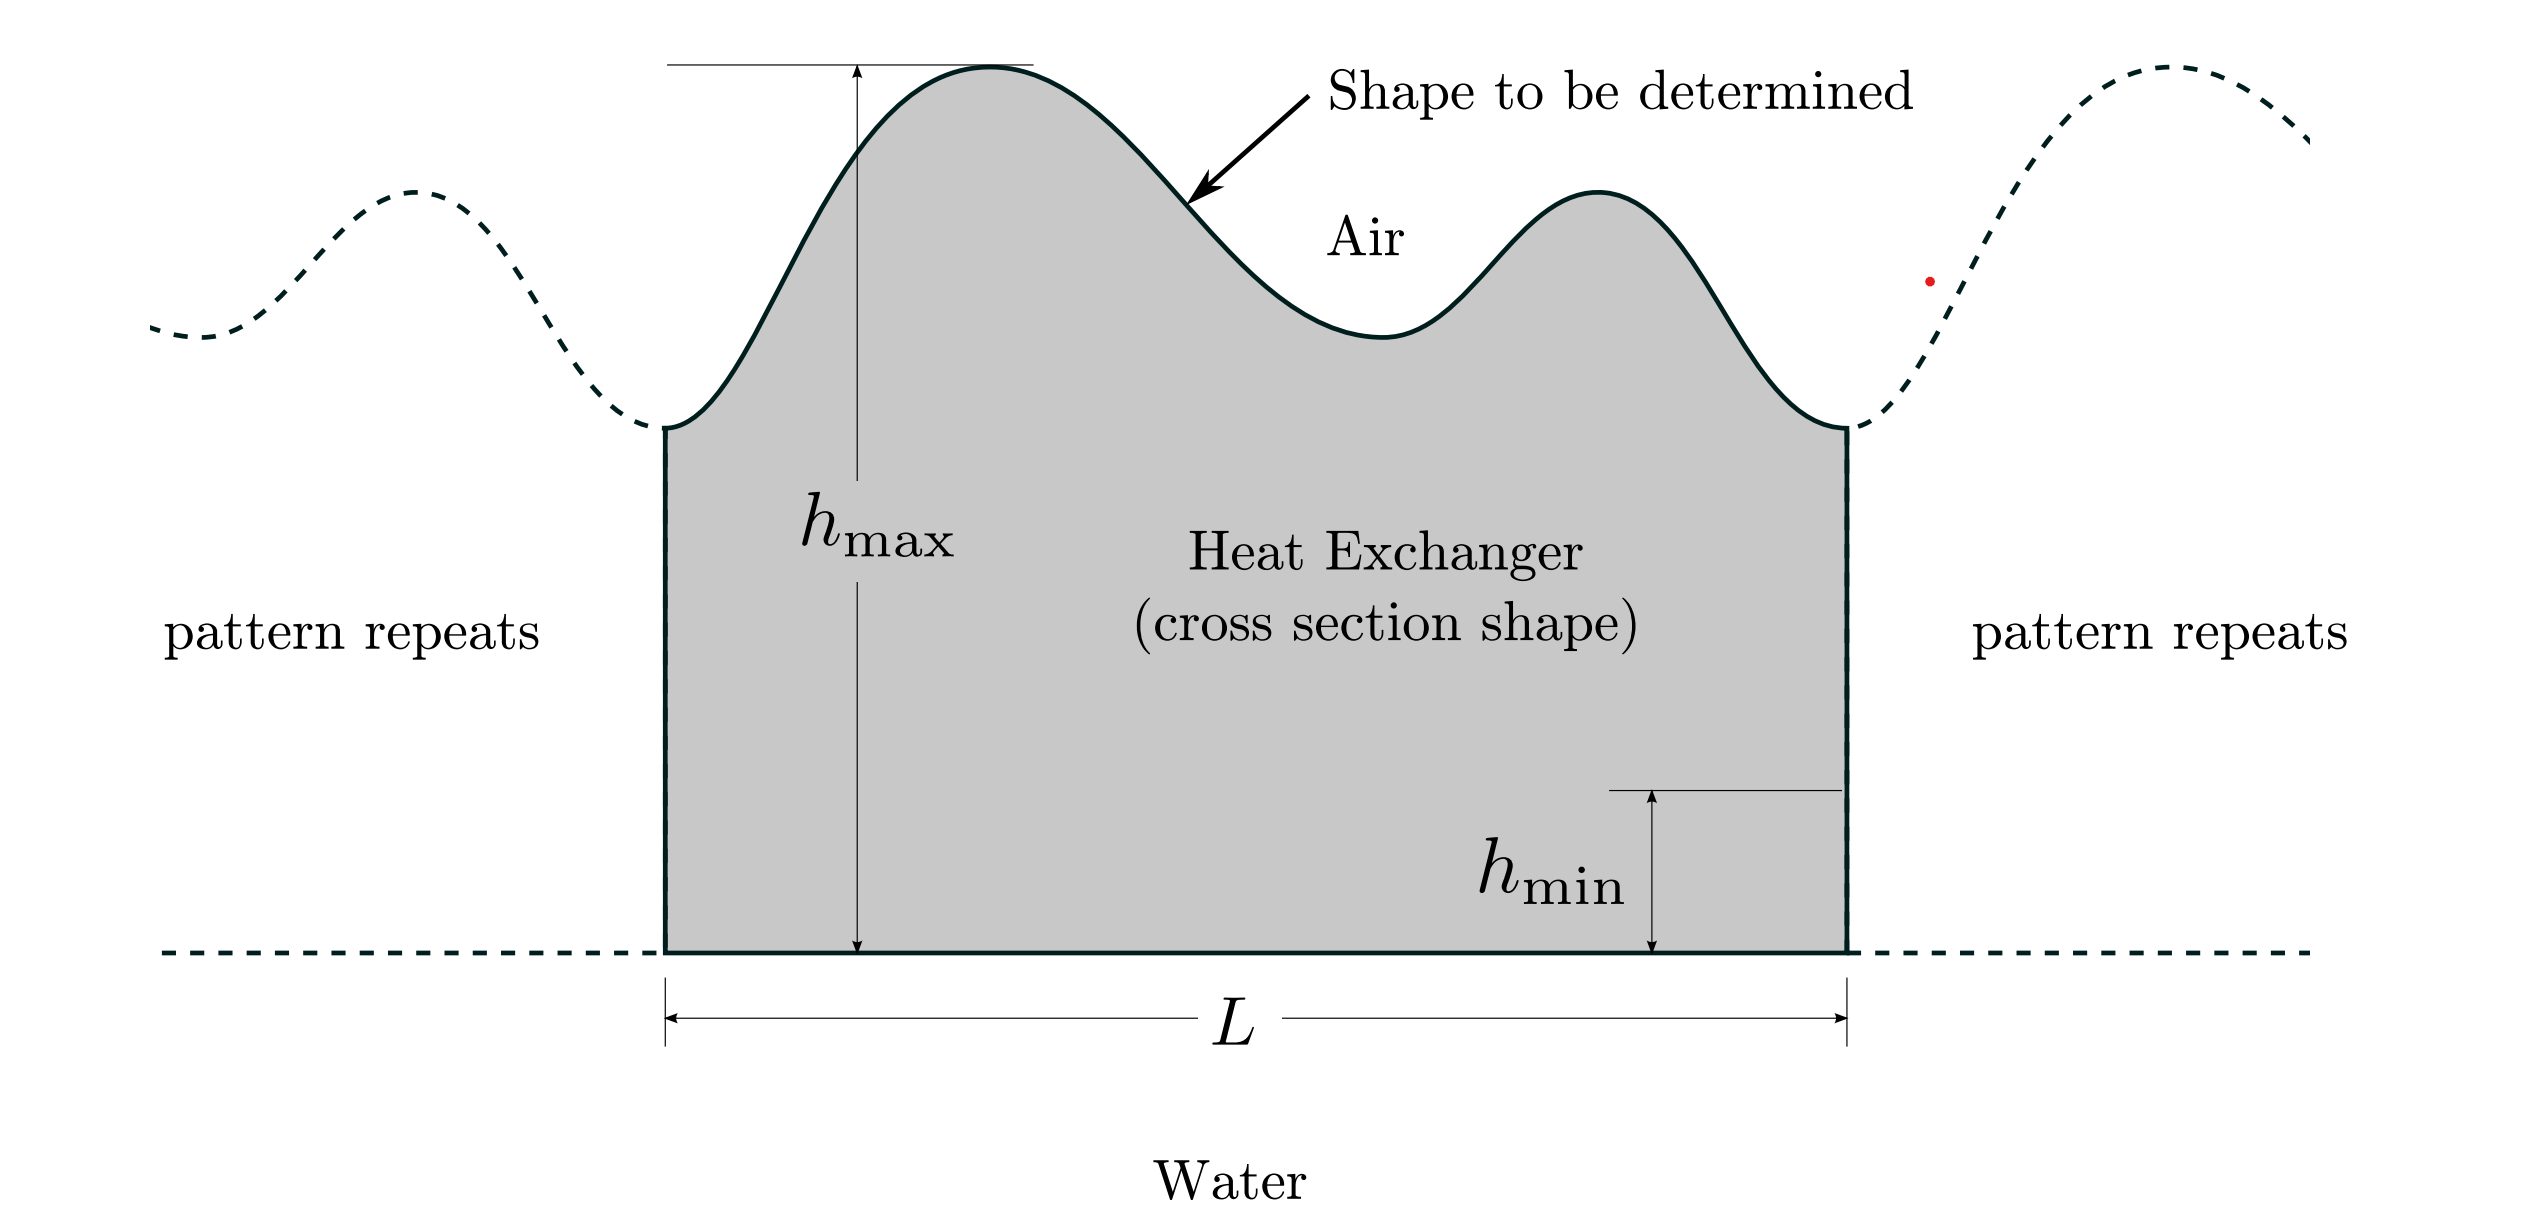
\includegraphics[width=0.75\linewidth]{introfig1.png}
    \caption{ Heat Exchanger Problem Illistration (\cite{lab1doc} Figure 1)}
    \label{fig:hxintro1}
\end{figure}
The objective of this project is to optimize the shape of the heat exchanger touching the air to maximize the heat flux per unit length transferred from the water to the air. The model geometry was parameterized and discretized (see section \ref{sec:parameterization} for more details) and applied to a descretized version of Fourier’s law to analyze the problem. The method chosen for the minimization problem was the SQP algorithm for the fmincon Matlab function (see section  \ref{sec:optimizationmethod} for more details). 

\section{Results}
The optimized shape of the heat exchanger with the chosen parameterization and the number of coefficients (16) is shown in Figure \ref{fig:cross}. To meet the minimum heat flux requirements from the rubric, the shape function requires more than ten design variables and Proffessor Hicken stated in class that less than twenty design variables should be used. With this in mind, sixteen design variables was chosen and the resulting design met requirements. This result makes sense, because it shows that the heat flux through the bottom of the heat exchanger is at its maximum when the surface area of the top of the heat exchanger is maximized. This is why many heat exchangers like the heat sinks used in computers use fins. 

\begin{figure}[h!]
    \centering
    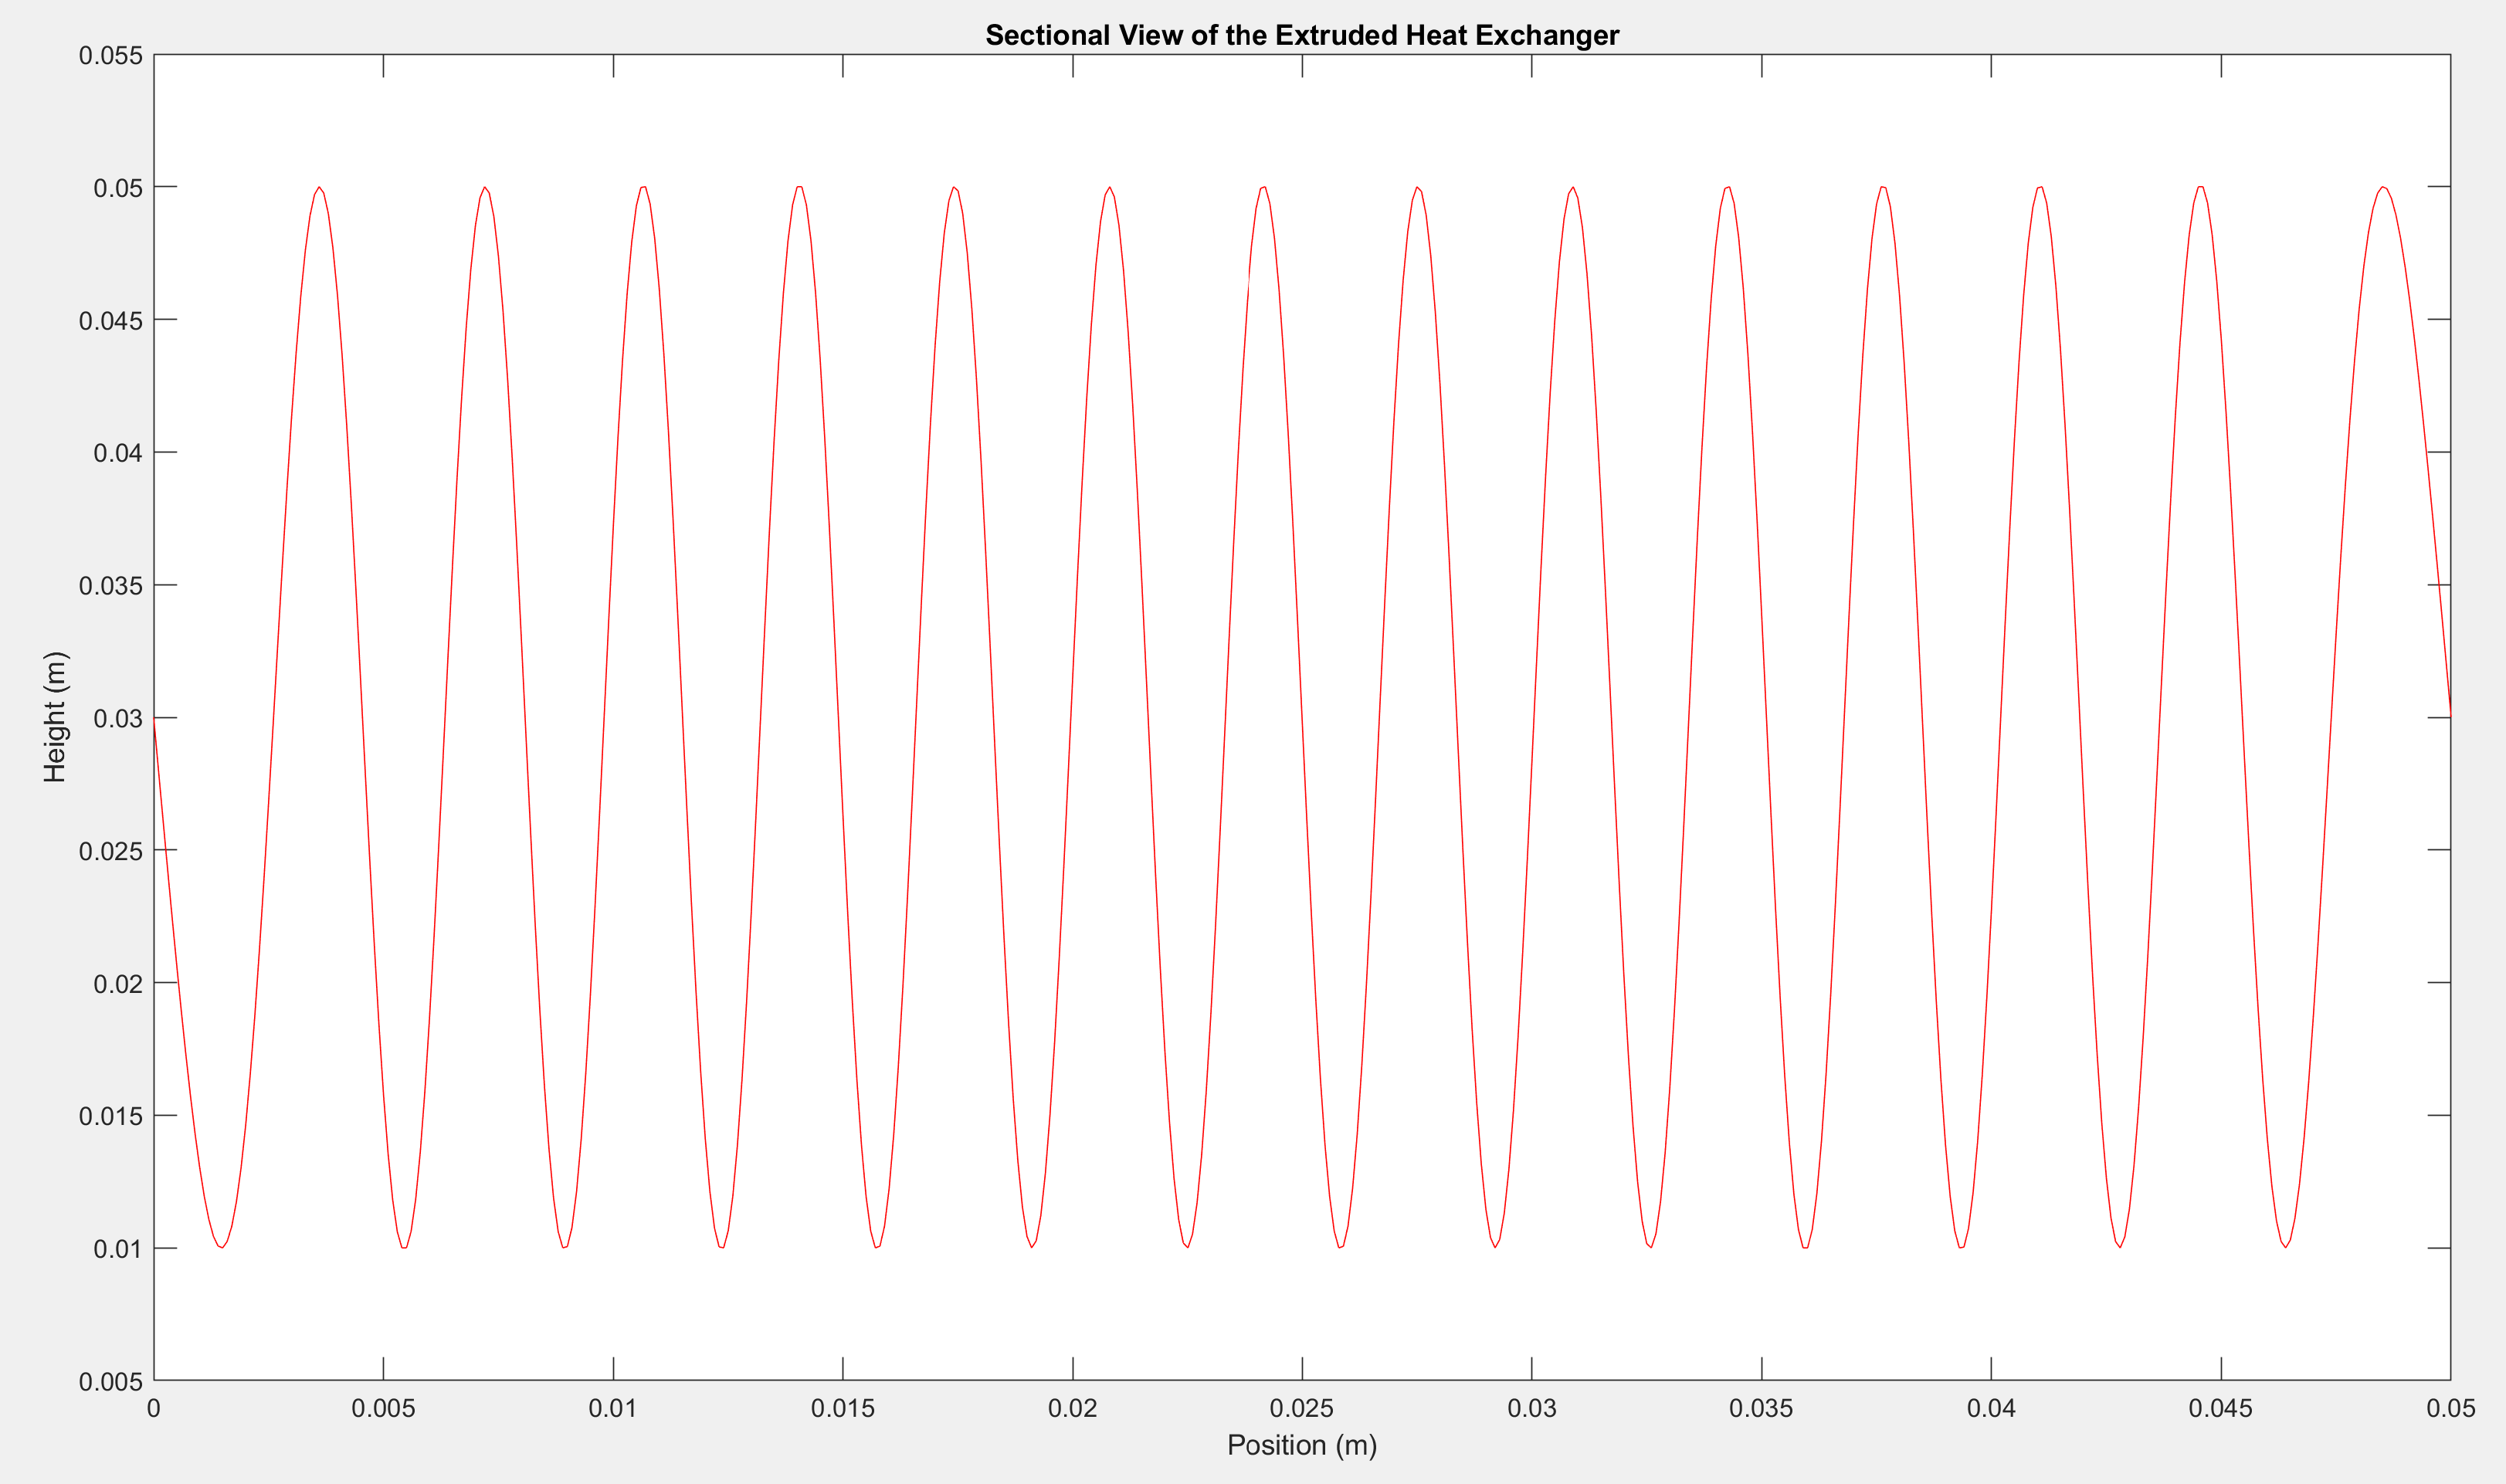
\includegraphics[width=0.75\linewidth]{crosssection.png}
    \caption{ Plot of the Heat Exchanger Cross Section }
    \label{fig:cross}
\end{figure}

The feasibility graph shows that the feasibility score of the current solution decreased rapidly over the first iteration and then stabilized over the remaining iterations as the First Order Optimality improved. The First Order Optimality graph shows a slow improvement over the iterations until the solver converged on a minimum causing a rapid improvement (see Figure \ref{fig:feas} both Feasibility and First-Order Optimality decreased by sixteen orders of magnitude over the itterations ).

\begin{figure}[h!]
    \centering
    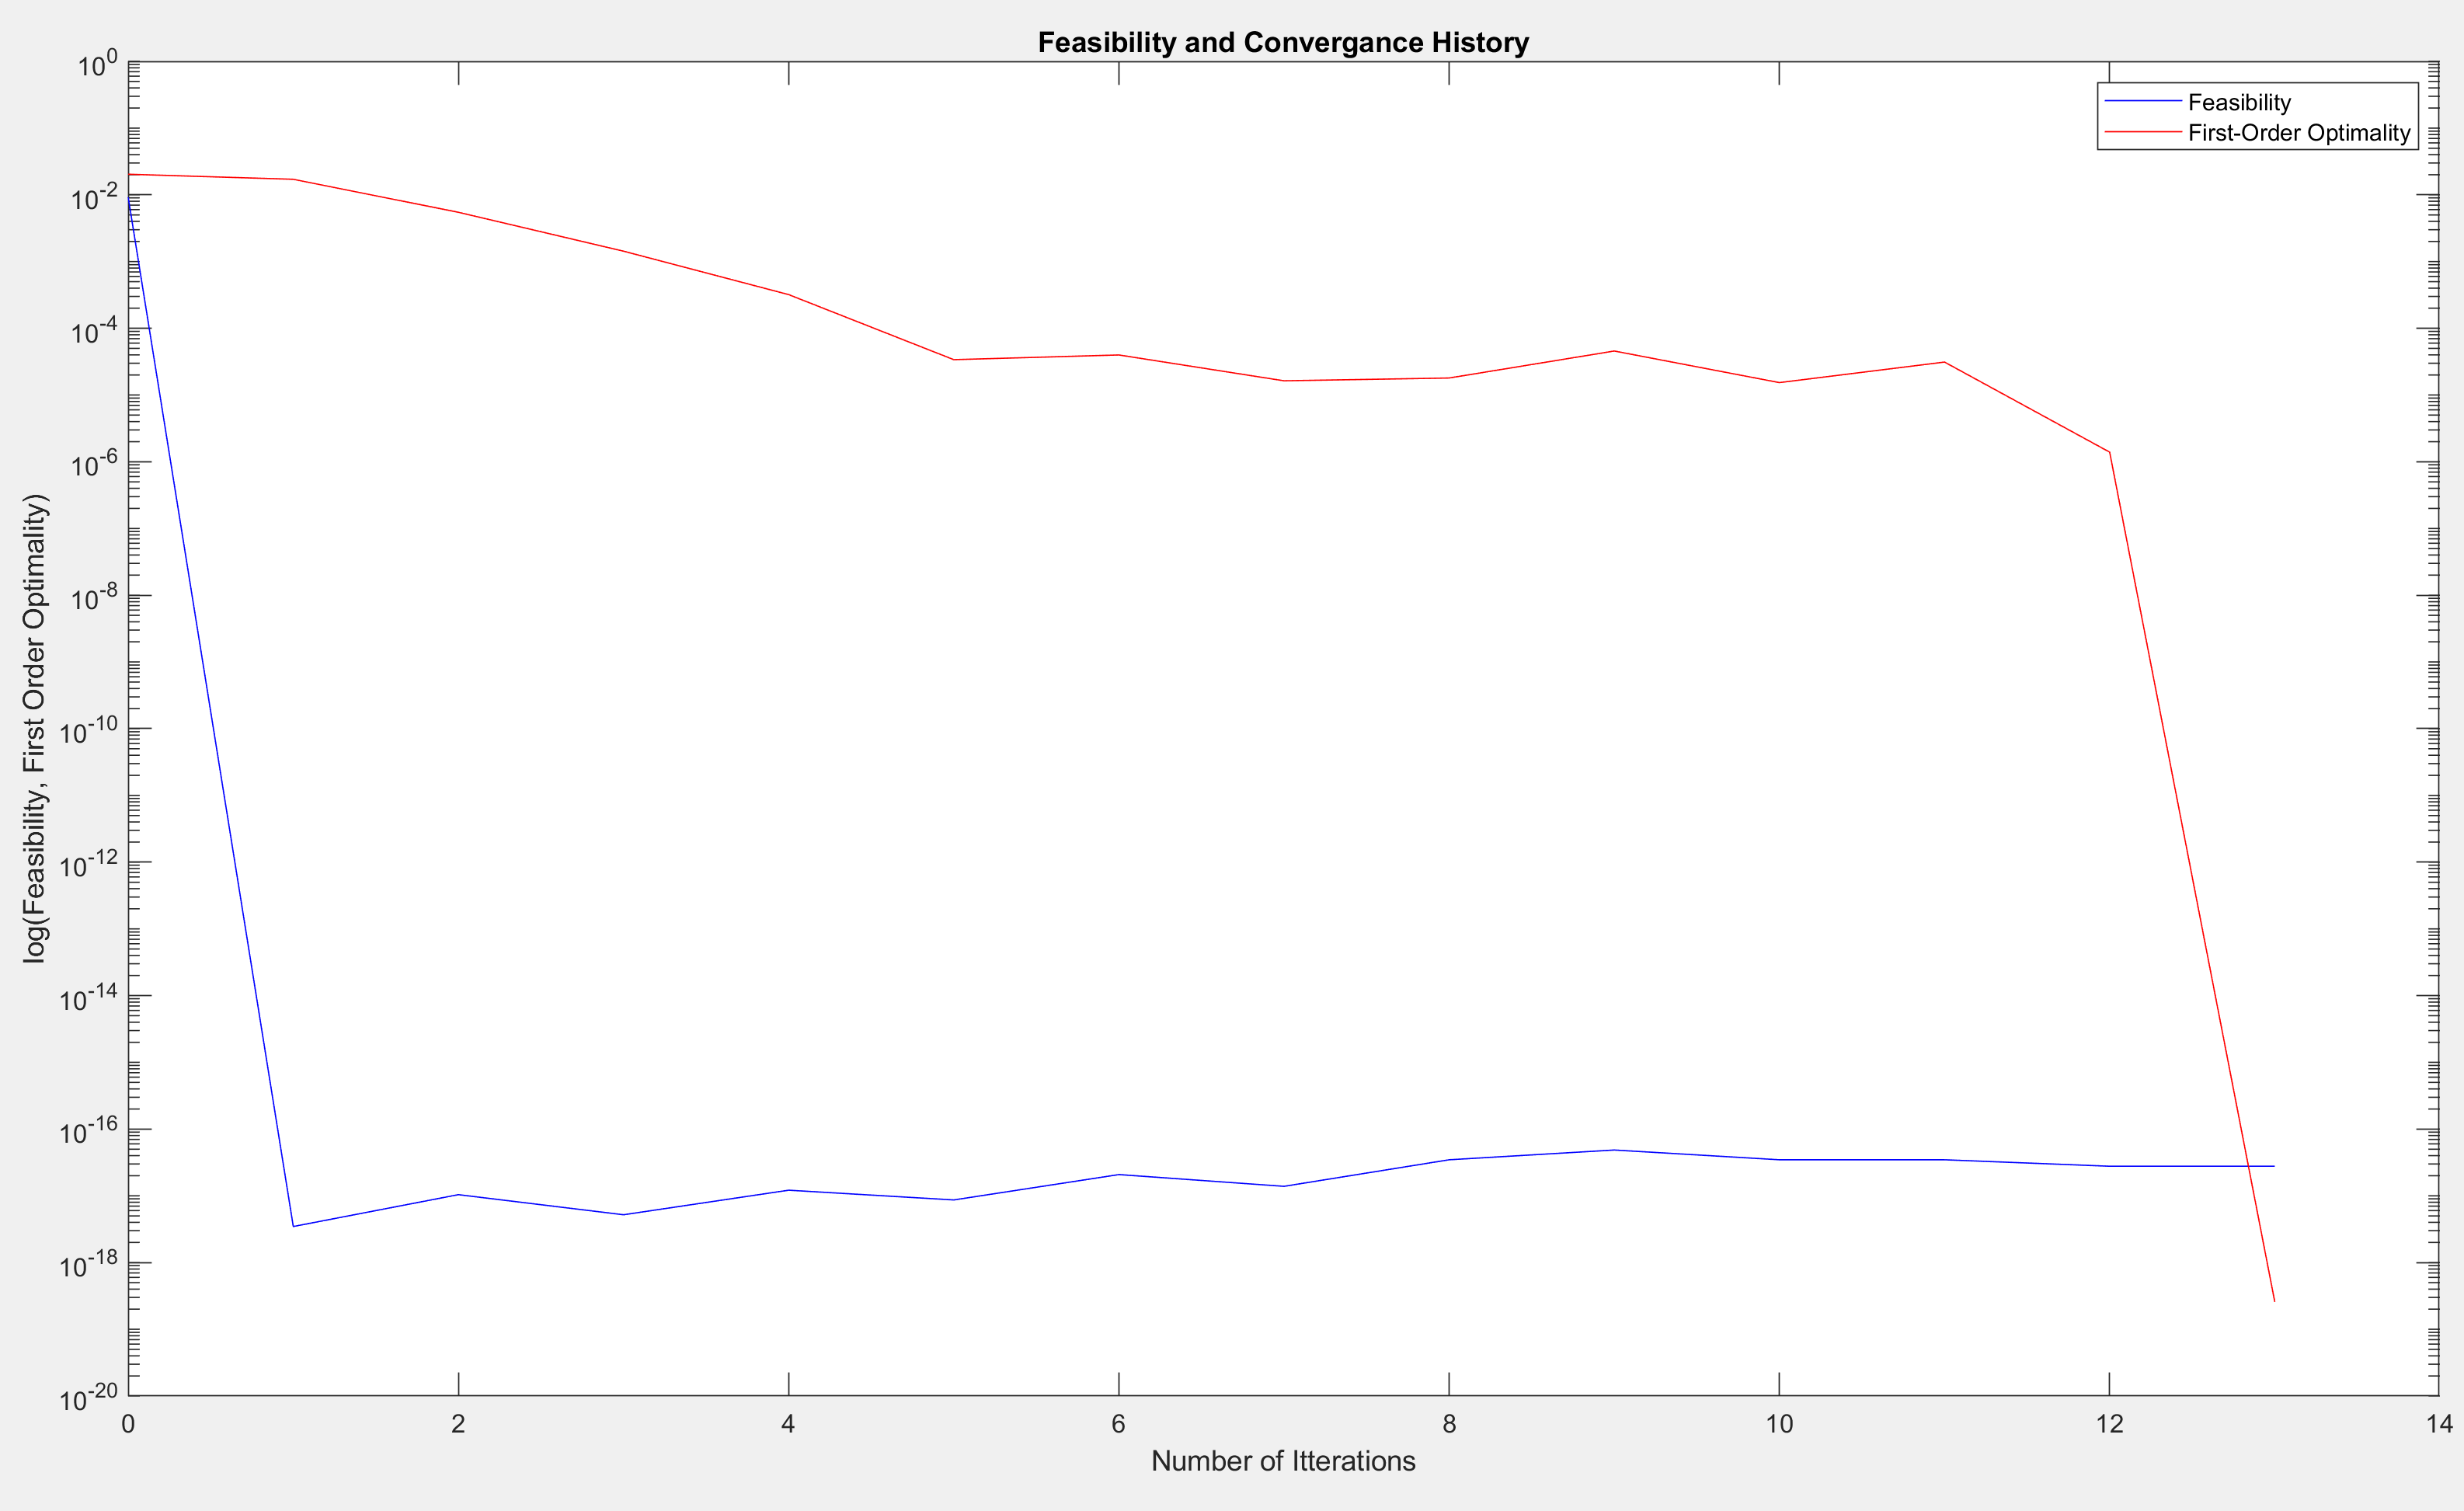
\includegraphics[width=0.75\linewidth]{feasibility.png}
    \caption{ The Feasibility and Convergence Plots }
    \label{fig:feas}
\end{figure}
\medskip
The convergence plot shown in Figure \ref{fig:conv} was calculated for the optimized shape function h(x) from Figure \ref{fig:cross}.  The plot shows jagged movement that quickly smooths out to an exponential curve approaching a value of about 4.5 kW/m as the number of segments increases. This behavior for small numbers of segments makes sense because for small numbers of segments the mesh doesn't adequately represent the temperature gradient so it doesn't behave as expected. Additionally, as the number of segments increases the calculated flux converges on the analytical solution as expected, because the series approximation of the integral becomes more accurate. The acceptable percent deviation is set to 5\% of the flux value as $N_{x}\rightarrow\infty$ because there are several curve fit equations for convection with similar accuracies.
\begin{figure}[h!]
    \centering
    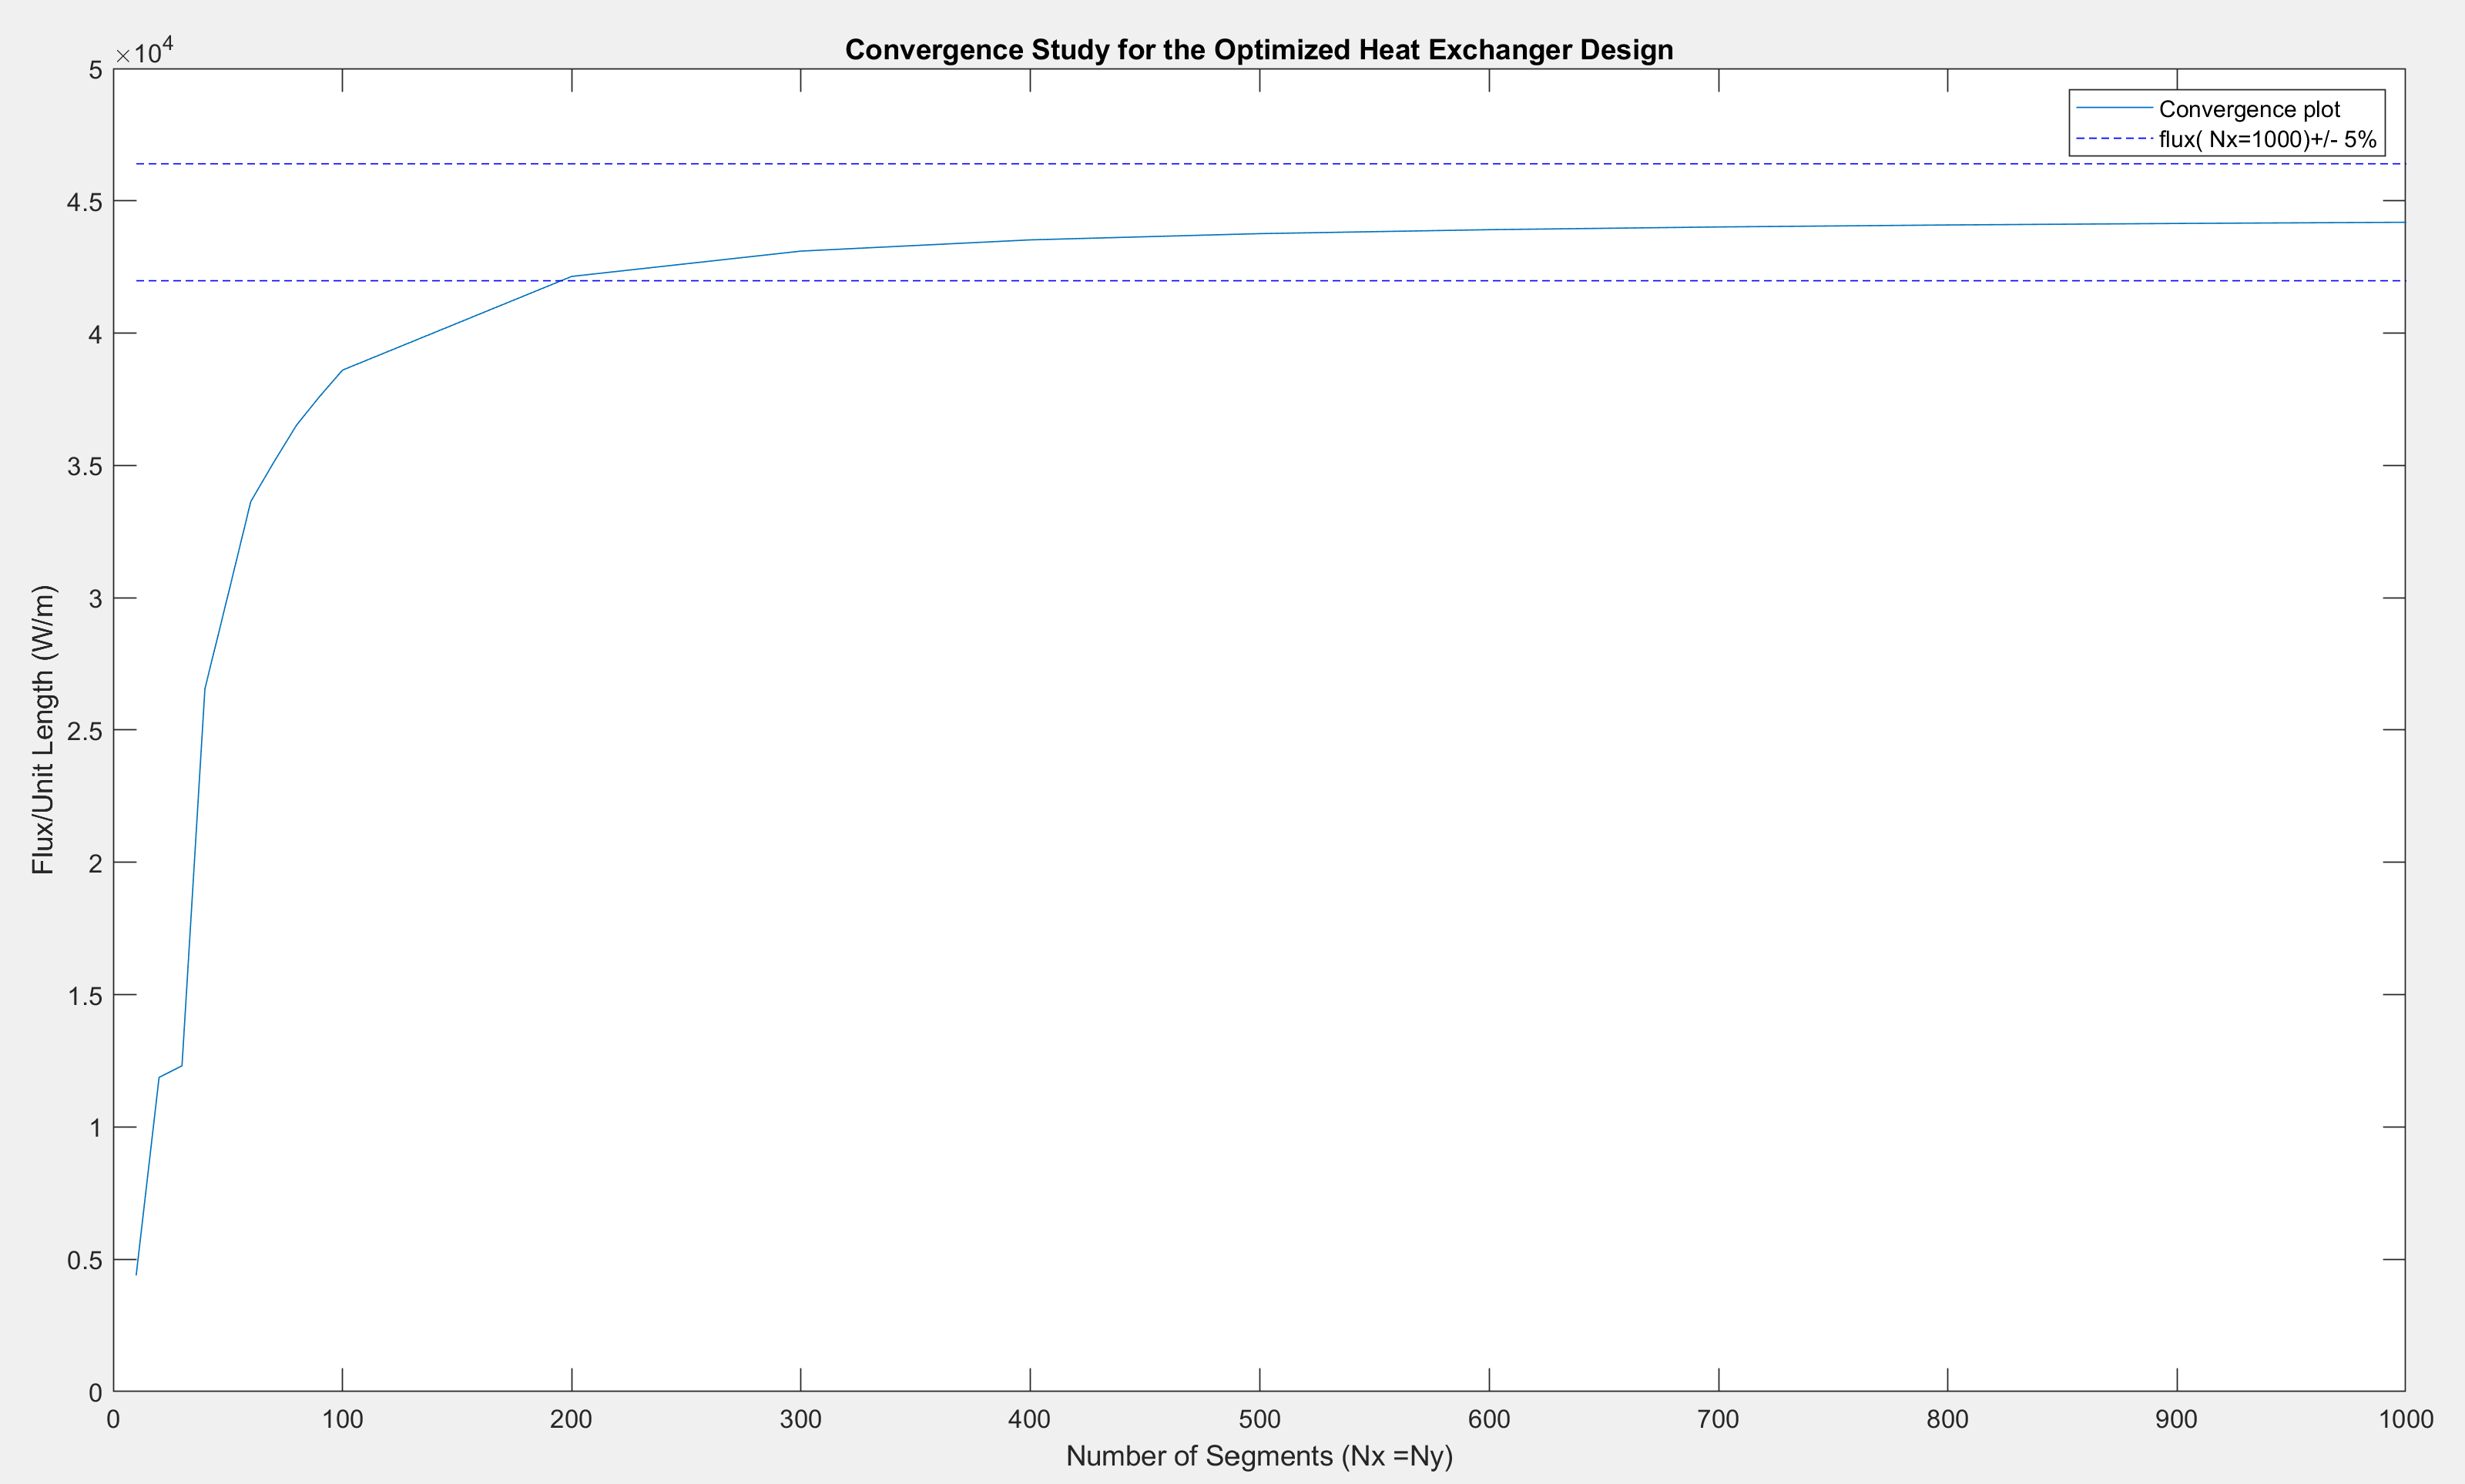
\includegraphics[width=0.75\linewidth]{converg.png}
    \caption{ Plot of the Flux vs Nx }
    \label{fig:conv}
\end{figure}
\section{Conclusions}
The implementation of the SQP optimization algorithm for this lab was successful. The resulting shape function for the optimized heat exchanger section profile made sense because it maximized the flux by maximizing the area in contact with the working fluids, which is how many similar devices are designed. The resulting calculated heat flux from the optimized heat exchanger was more than four times greater than the baseline design ($44190 > 28000 $ W/m) while remaining within the problem constraints. 

 Basic optimization algorithms, such as the ones used in this lab, can be powerful tools for understanding the complex interactions between different design variables in engineering design problems and balancing the design variables to arrive at an optimal solution. Understanding how these algorithms work and the trade-offs between accuracy and run time shown in the convergence study is important when utilizing these algorithms to solve problems. 

\addcontentsline{toc}{section}{References}
\printbibliography
\newpage
\section{Appendix}

\lstset{language=Matlab,%
    %basicstyle=\color{red},
    breaklines=true,%
    morekeywords={matlab2tikz},
    keywordstyle=\color{blue},%
    morekeywords=[2]{1}, keywordstyle=[2]{\color{black}},
    identifierstyle=\color{black},%
    stringstyle=\color{mylilas},
    commentstyle=\color{mygreen},%
    showstringspaces=false,%without this there will be a symbol in the places where there is a space
    numbers=left,%
    numberstyle={\tiny \color{black}},% size of the numbers
    numbersep=9pt, % this defines how far the numbers are from the text
    emph=[1]{for,end,break},emphstyle=[1]\color{red}, %some words to emphasise
    %emph=[2]{word1,word2}, emphstyle=[2]{style},    
}
\subsection{calcHeight.m}
\label{sec:calcHeight}
\lstinputlisting{calcHeight.m}
\newpage
\subsection{objective.m}
\label{sec:objective}
\lstinputlisting{objective.m}
\newpage
\subsection{run\_opt.m}
\label{sec:runOpt}
\lstinputlisting{run_opt.m}
\newpage
\subsection{plots.m}
\label{sec:plots}
\lstinputlisting{plots.m}
\subsection{fmincon Output}
\label{sec:fincon}
\begin{figure}[h!]
    \centering
    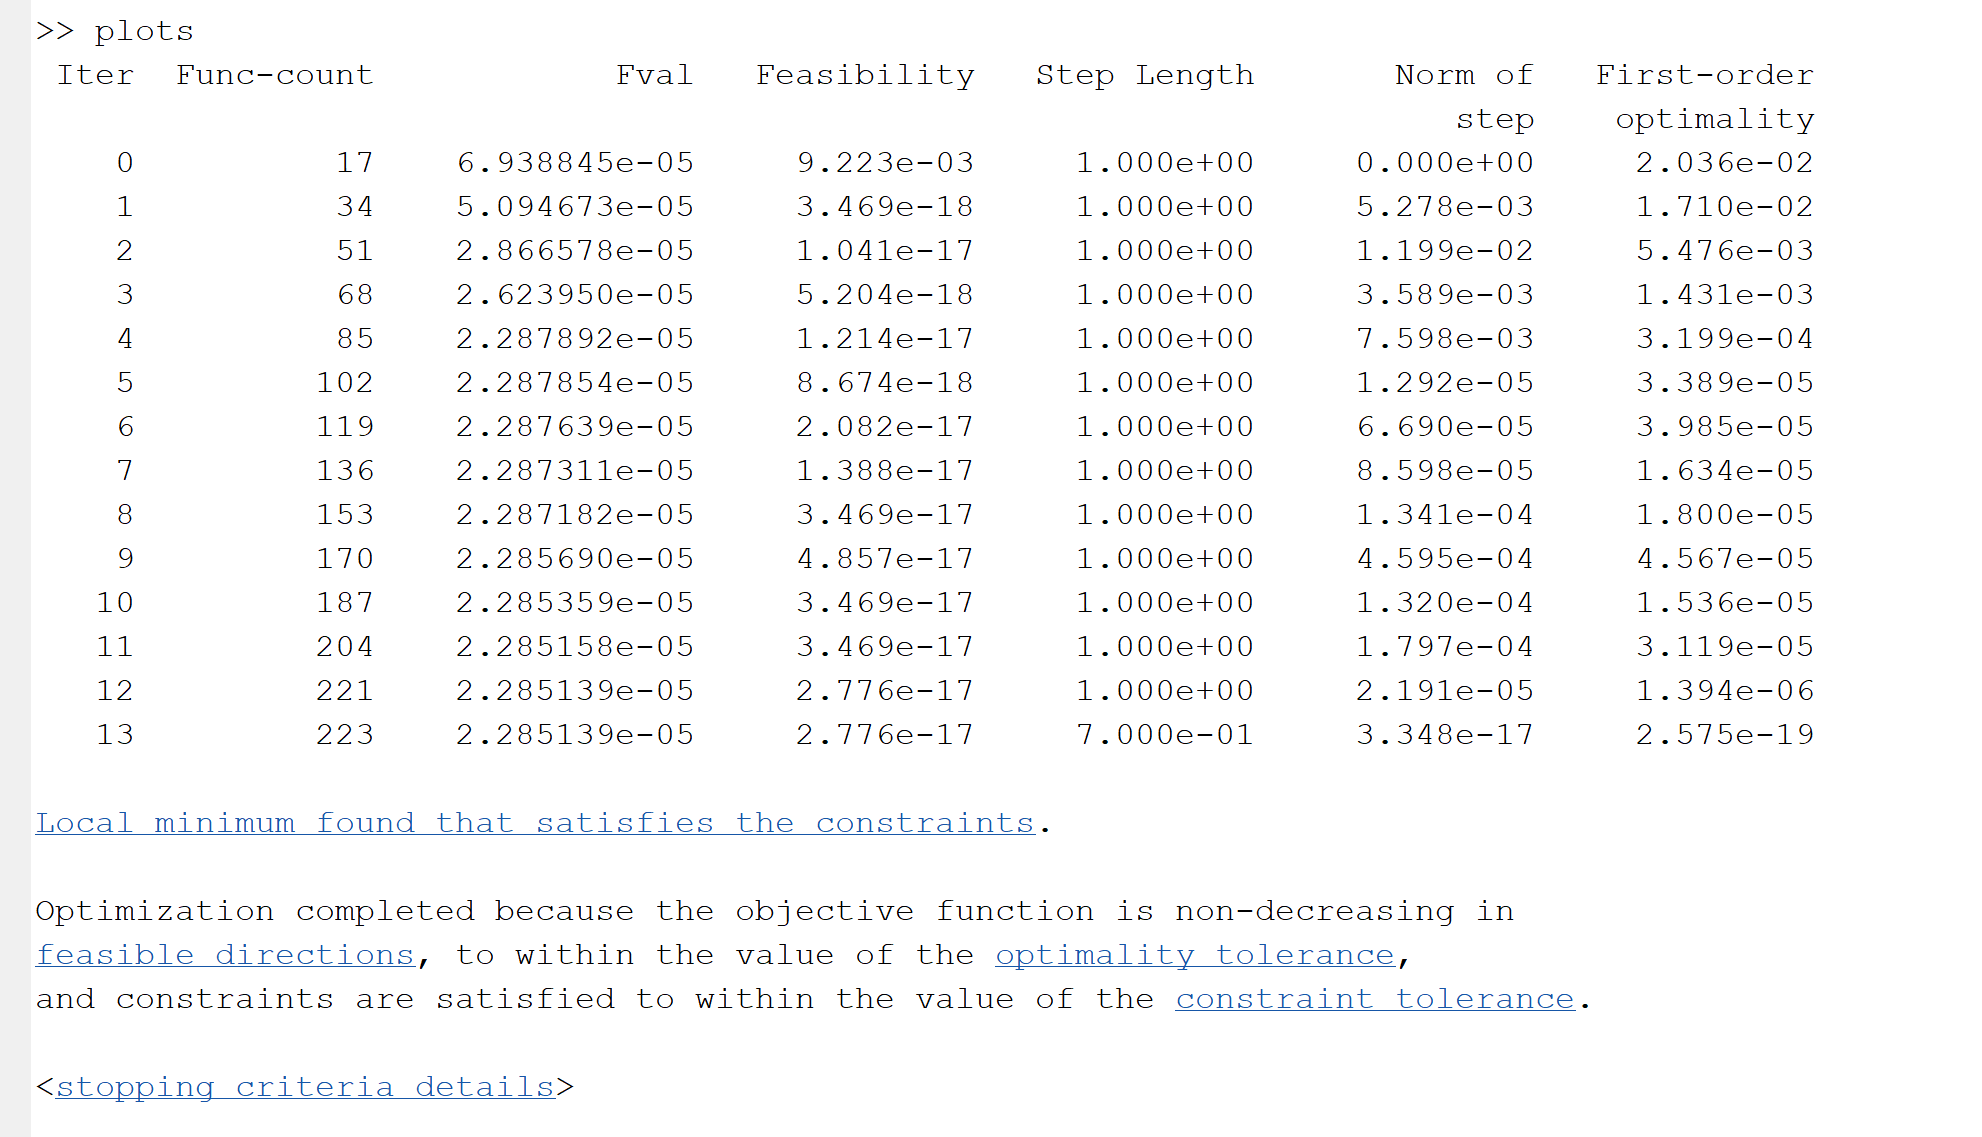
\includegraphics[width=0.75\linewidth]{fminconoutput.png}
    \caption{ The Outpt of fmincon }
    \label{fig:fmincon}
\end{figure}
\end{document}